\documentclass[a4paper,10pt]{article}
\usepackage[utf8]{inputenc}
%\usepackage{../outlines_pkg/outlines}
\usepackage{amsmath}
\usepackage{amssymb}
\usepackage{amsthm}
\usepackage{enumerate}
\usepackage[square,sort,numbers]{natbib}
\usepackage{xspace}
\usepackage{graphicx}
\usepackage{subcaption}

\title{Grid USO algorithms}
\author{Antonis, Bernd, Jerri, Luis, Malte}

\newtheorem{observation}{Observation}
\newtheorem{lemma}{Lemma}
\newtheorem{definition}{Definition}
\newtheorem{corollary}{Corollary}
\newtheorem{theorem}{Theorem}

%%%%%%%%%%%%%%%%%%%%%%%%%%%%%%%%%%%%%%%%%%%%%%%%%%%%%%%%%%%%%%%%%%%%%%
% Setup margin comments. If you want to ignore them, then comment the other part out.
\newcommand{\JN}[1]{\marginpar{\parbox{4cm}{{\small {\bf JN:} #1}}}} %Jerri
\newcommand{\LB}[1]{\marginpar{\parbox{4cm}{{\small {\bf LB:} #1}}}} %Luis
\newcommand{\MM}[1]{\marginpar{\parbox{4cm}{{\small {\bf MM:} #1}}}} %Malte
\newcommand{\AT}[1]{\marginpar{\parbox{4cm}{{\small {\bf AT:} #1}}}} %Antonis
\newcommand{\BG}[1]{\marginpar{\parbox{4cm}{{\small {\bf BG:} #1}}}} %Bernd
%\newcommand{\JN}[1]{}

%%%%%%%%%%%%%%%%%%%%%%%%%%%%%%%%%%%%%%%%%%%%%%%%%%%%%%%%%%%%%%%%%%%%%%

\newcommand{\indegree}{refined in-degree\xspace}
\newcommand{\ind}{\ensuremath{\mathrm{ind}}}

\begin{document}

\maketitle 

\begin{abstract}
Deterministic algorithm for two dimensional grid USOs.
\end{abstract}

\section{Introduction}

Let $X$ and $Y$ be any finite sets and let $K_X$ denote the complete graph on the vertex set $X$. The product graph $K_X\times K_Y$ is called the \emph{$X\times Y$-grid} or simply a \emph{grid}. For $m,n \in \mathbb{N}$ an $m\times n$ grid is any grid $K_X\times K_Y$ with $|X| = m$ and $|Y| = n$. The vertex set of the grid $K_X\times K_Y$ is $X\times Y$ and $(v_x,v_y),(w_x,w_y) \in X\times Y$ are adjacent if either $v_x = w_x$ and $v_y \not= w_y$ or $v_x \not= w_x$ and $v_y = w_y$. In the first case we call the edge \emph{vertical} and in the latter we call it \emph{horizontal}. This terminology comes from identifying the elements of $X$ and $Y$ with real numbers and then embedding the vertices on the Euclidian plane. 

An induced subgraph of a grid is called a \emph{subgrid} if it is also a grid. Any subgrid of an $X\times Y$-grid is an $I\times J$-grid where $I \subseteq X$ and $J \subseteq Y$. If a grid is oriented then a subgrid inherits the orientation. A vertex in an oriented graph is called a \emph{sink} if all its incident edges are incoming. An orientation of a grid is a \emph{unique sink orientation}, or \emph{USO} for short, if all its subgrids have a unique sink. In a grid unique sink orientation $G$ the \emph{\indegree} of a vertex $v \in G$ is an ordered pair $\ind (v) \in \{0,1,\ldots,|X|-1\}\times \{0,1,\ldots,|Y|-1\}$ which specifies the number of incoming horizontal and vertical edges of $v$ respectively. 

Given a grid USO the task is to find the global sink. The USO is given via a vertex oracle: for each \emph{vertex query} the oracle reveals the orientations of the edges adjacent to the vertex. The question is, how many vertex queries suffice to find the sink of a grid USO of certain size?

We define a partial order of vertices in a grid unique sink orientation $G$ as follows. For any two vertices $v,w \in G$ consider the smallest subgrid containing both $v$ and $w$. We say that $w \succeq v$ if there is a path from $w$ to $v$ in this subgrid. Notice that not necessarily all vertices are comparable.



\begin{lemma}[Product construction]
 Let $G$ be an $X\times Y$-grid USO for some sets $X$ and $Y$ and let $A \subset 2^X$ and $B \subset 2^Y$ be partitions of $X$ and $Y$ respectively. Let $H$ be an $A\times B$-grid. \JN{See Malte's 4$\times$4 lower bound for a possible way to define this.}
\end{lemma}


\section{The algorithm}

\begin{lemma}
 Given an $n\times n$ grid USO we can find a vertex with a \indegree $(a,b)$ satisfying $a, b \geq \frac{n}{4} - 1$ by using $\mathcal{O}(n)$ vertex queries.
\end{lemma}

\begin{proof}
 First, query the diagonal i.e. the vertices $v_i = (i,i)$, $i = 1,\ldots,n$. We can assume that $j < i$ implies that either $v_j \succeq v_i$ or $v_j$ and $v_i$ are incomparable; otherwise just rename the coordinates. \JN{Sorting overhead which is not needed for the actual algorithm, but only for the analysis.} Then, each $v_i$ has at least $i-1$ incoming edges. This can be seen by looking at all vertices $v_j$ with $j < i$. Either $v_j \succeq v_i$ or they are not comparable, but in both cases there is one incoming edge towards $v_i$ in the $2\times 2$ subgrid containing both $v_i$ and $v_j$. 
 
 Now let $V = \{v_{\lceil n/2 \rceil},\ldots,v_n\}$. For each vertex in $V$ record if the majority of its incoming edges are horizontal or vertical and call such a vertex horizontal or vertical respectively. By symmetry we can assume that there are more vertical vertices in $V$ and let $V' \subseteq V$ be the set of vertical vertices. Note that $|V'| \geq \frac{n-\lceil n/2\rceil + 1}{2} \geq \frac{n}{4}$ and each vertex in $V'$ has at least $\frac{\lceil n/2\rceil-1}{2}$ incoming vertical edges. 
  Let $v_k \in V'$ be the vertical vertex with maximal index $k$. \JN{This should be maybe written using the product construction.} Query all the vertices that are in the same row as $v_k$ and in the same column with some vertex from $V'$. Let $v^*$ be the sink of the $|V'|\times 1$ subgrid formed by these evaluated vertices (including $v_k$). Let $(a,b)$ be the \indegree of $v^*$. We claim that $a, b \geq \frac{n}{4} - 1$. Firstly, Note that $v^*$ has incoming edges from all of the other vertices in the $|V'|\times 1$ subgrid we evaluated, so $a \geq |V'|-1 \geq \frac{n-\lceil n/2\rceil + 1}{2} - 1 \geq \frac{n}{4} - 1$. Secondly, there is a vertex $v \in V'$ that is in the same column as $v^*$.
  The situation is depicted in Figure~\ref{fig:seedlem1}.
  \begin{figure}[htbp] 
  	\centering
  	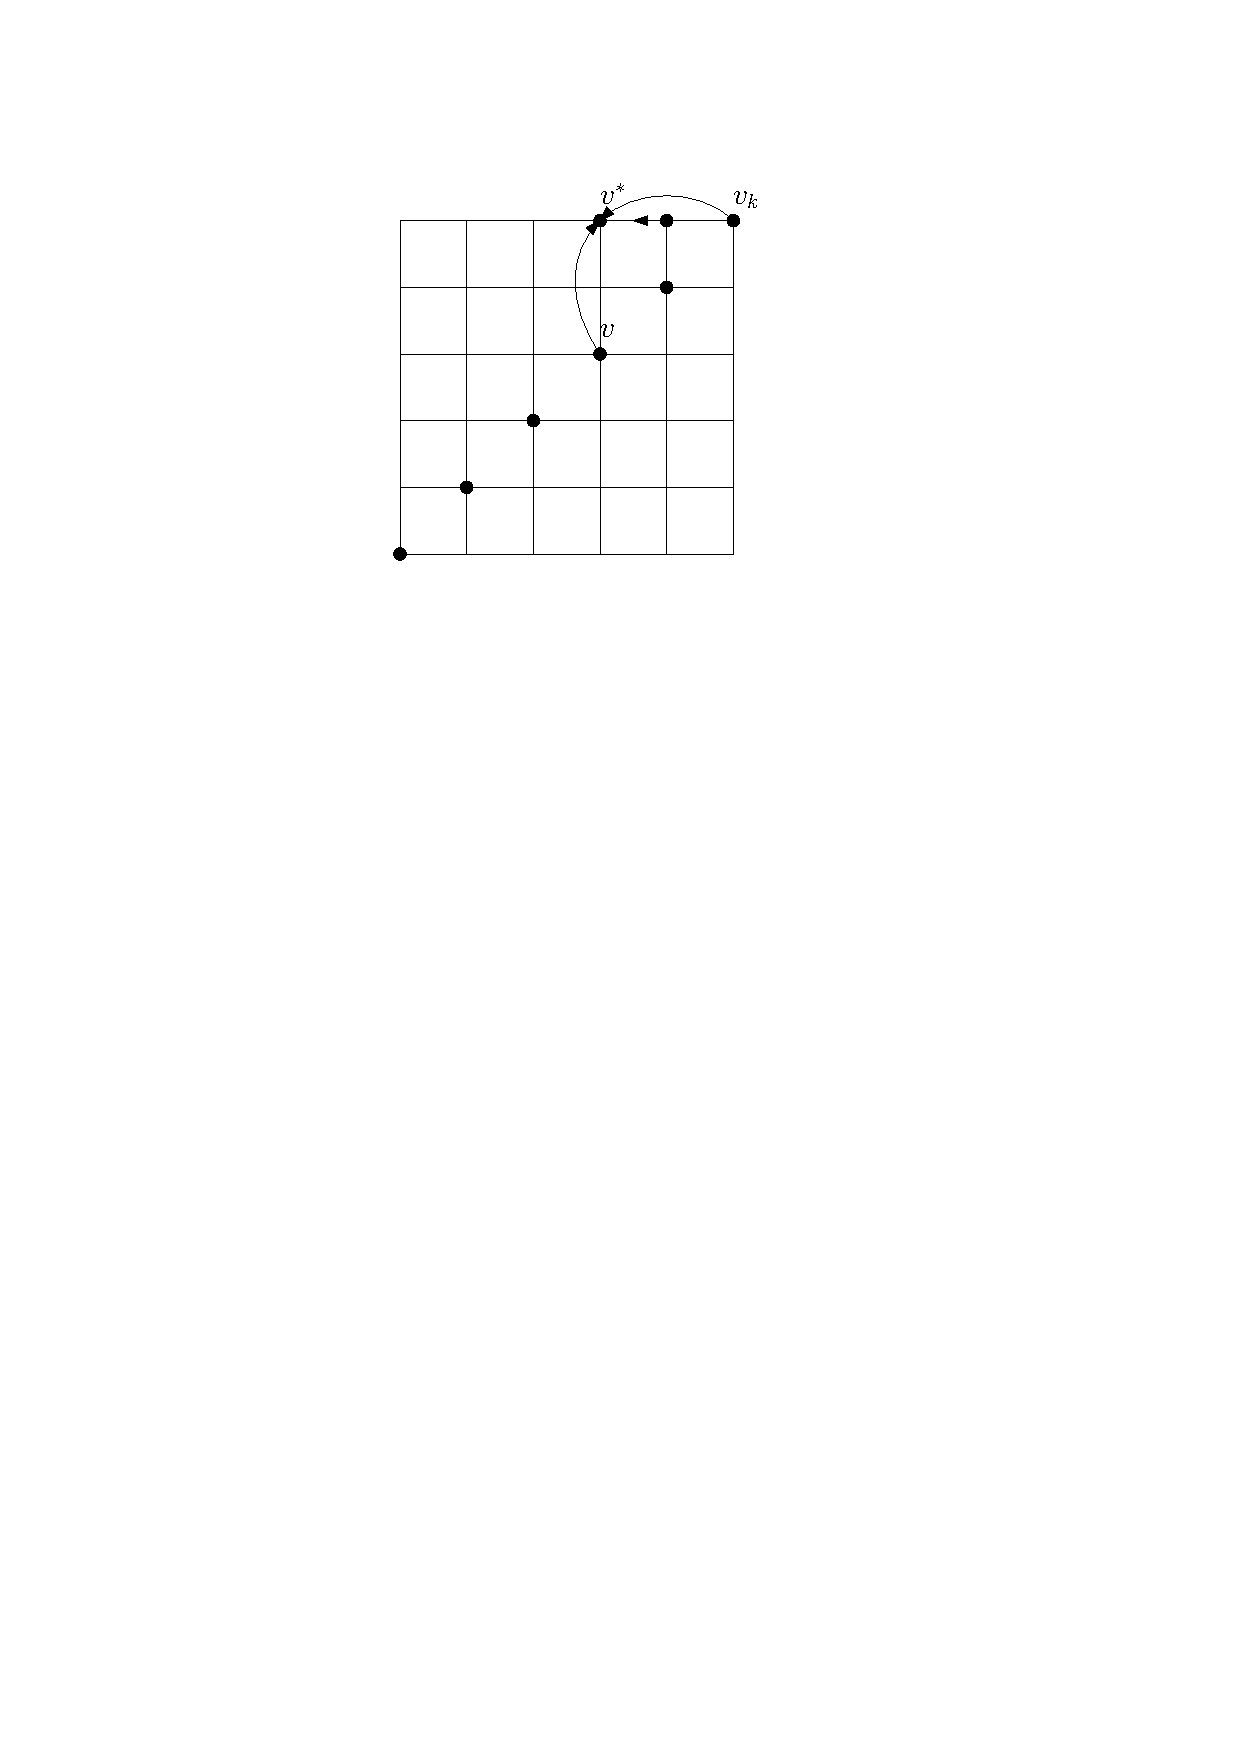
\includegraphics[scale=0.7]{seedlemma_fig1.pdf}
  	\caption{In this figure only a subset of the edges of the grid appears. The vertices that are marked with discs are the ones evaluated.} 
  	\label{fig:seedlem1}
  \end{figure}
   If we can show that there is an edge from $v$ to $v^*$, then by acyclicity $v^*$ has at least one more incoming vertical edge as compared to $v$, therefore establishing that $b \geq \frac{\lceil n/2\rceil-1}{2} + 1 \geq \frac{n}{4} \geq \frac{n}{4} - 1$. To show that there is an edge from $v$ to $v^*$ there are two cases. In the first case $v \succeq v_k$ and because $v_k \succeq v^*$ we have due to transitivity that $v \succeq v^*$. In the second case $v$ and $v_k$ are incomparable. Then, the edge between $v$ and $v^*$ has to be oriented towards $v^*$. This is because otherwise we would have that $v_k \succeq v$. We give illustrations of the two cases in Figure~\ref{fig:seedlem2}; the proof is finished. 
   \begin{figure}[htbp] 
       \centering
       \begin{subfigure}[b]{0.4\textwidth}
           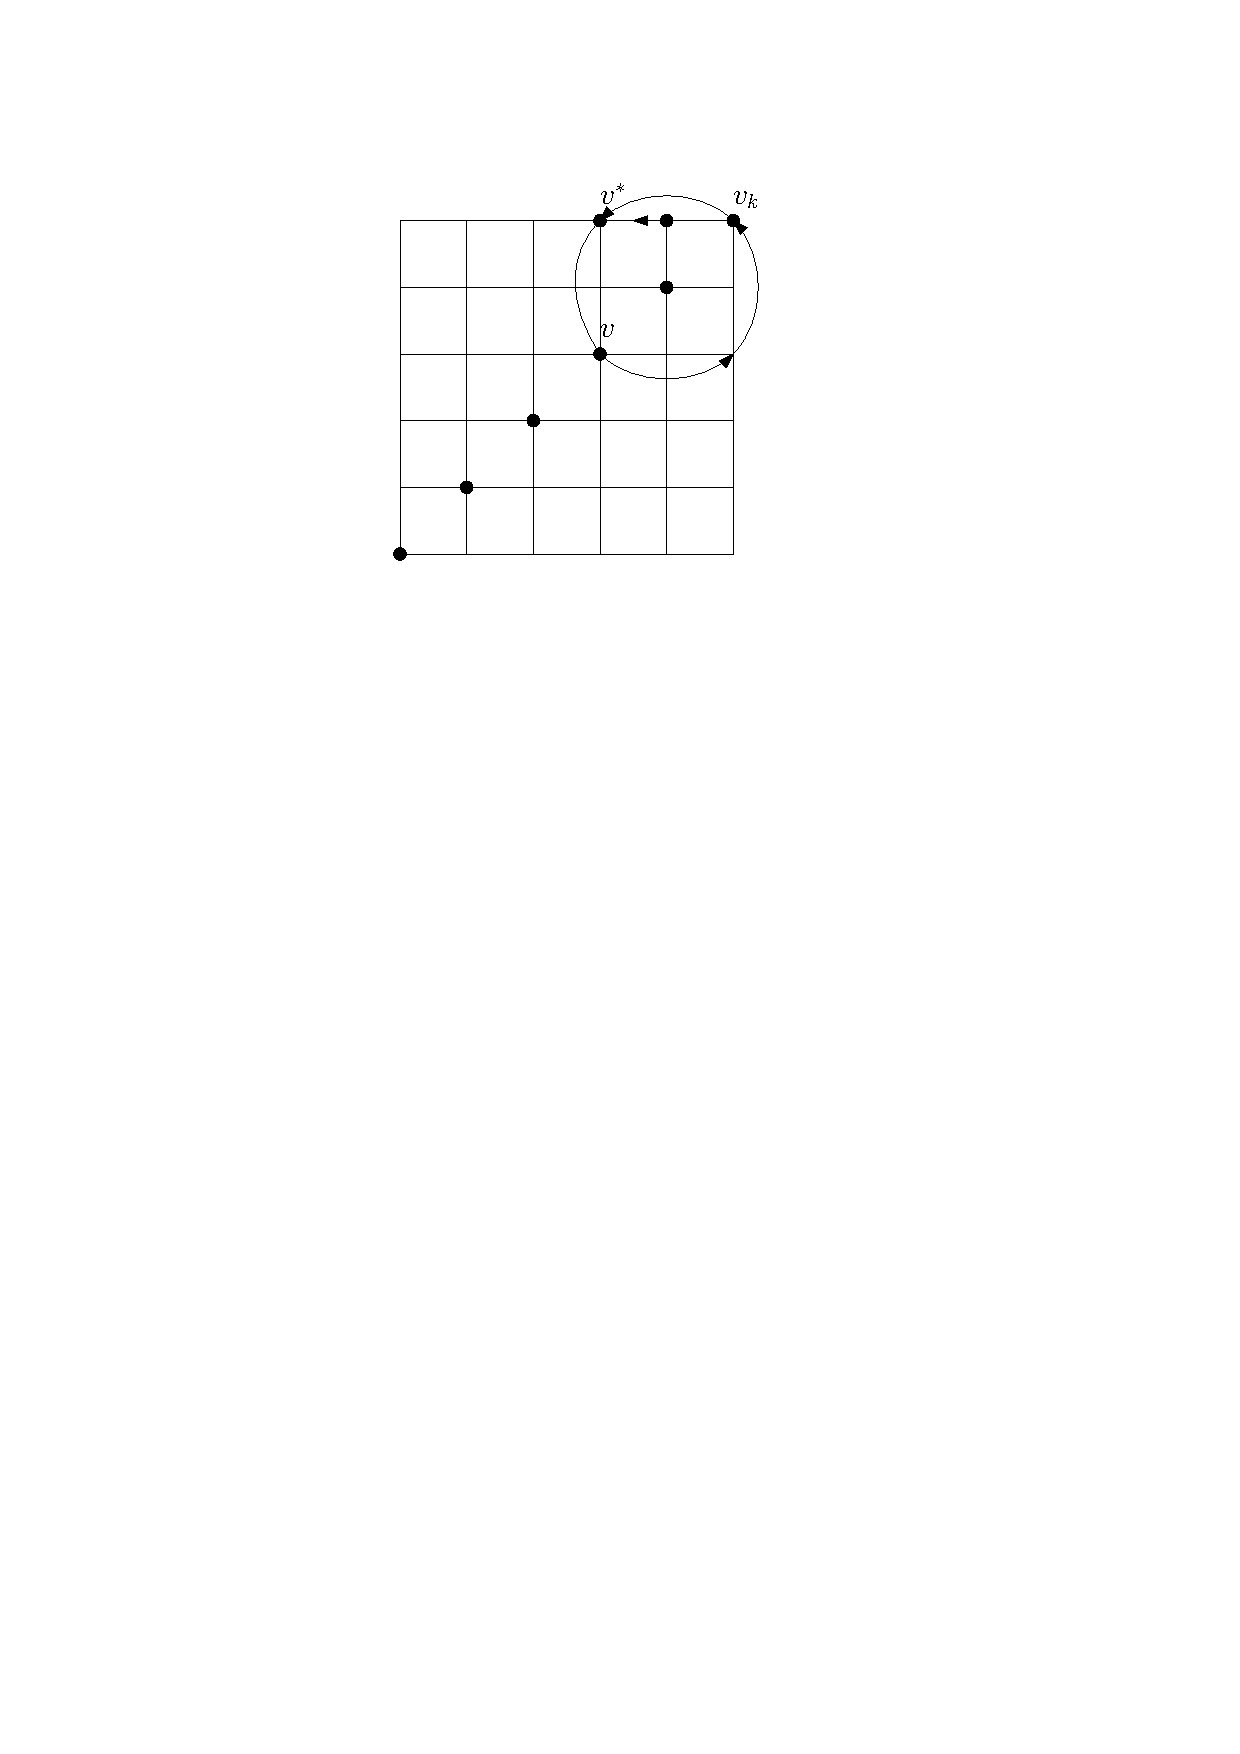
\includegraphics[scale = 0.7]{seedlemma_fig2_cas1.pdf}
           \caption{$v \succeq v_k$}
       \end{subfigure}
       \qquad \qquad
       \begin{subfigure}[b]{0.4\textwidth}
           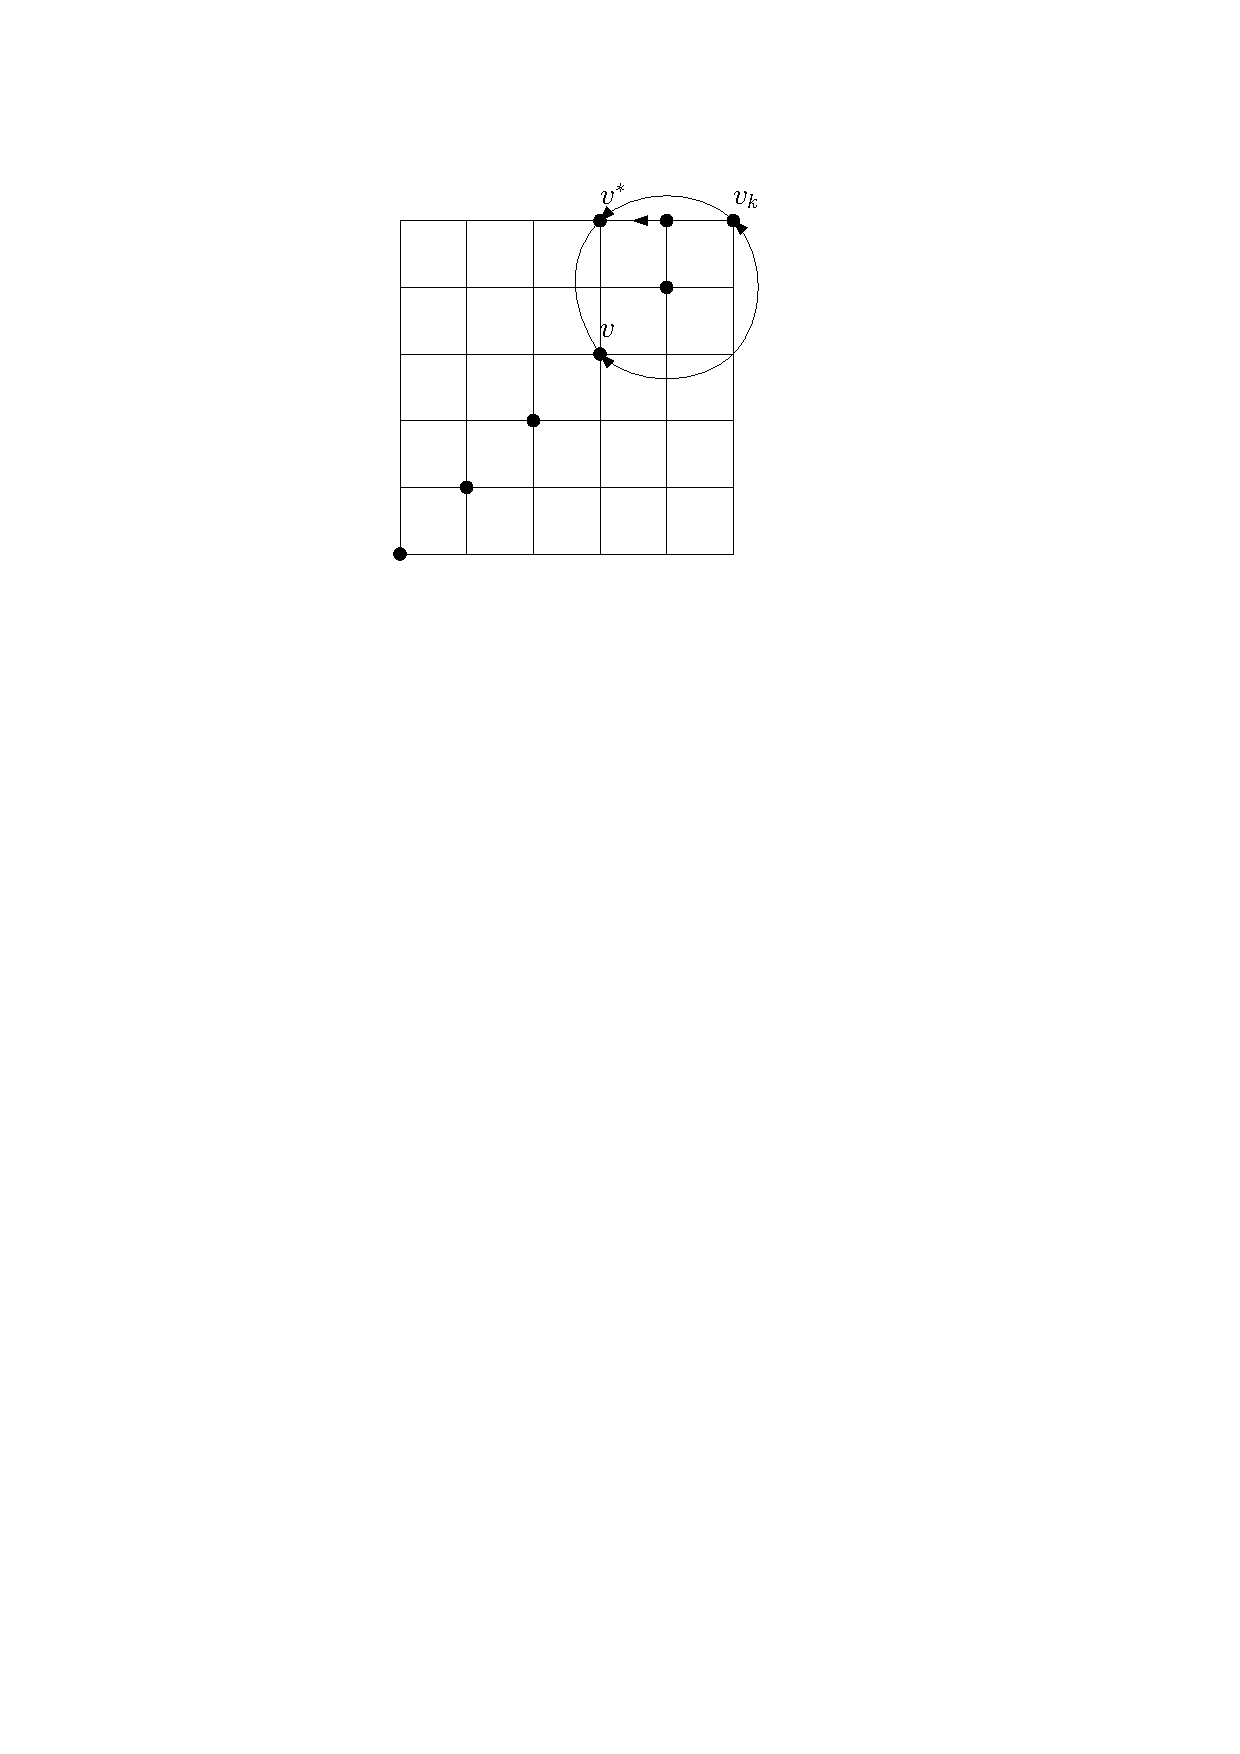
\includegraphics[scale = 0.7]{seedlemma_fig2_cas2.pdf}
           \caption{$v$ and $v_k$ are incomparable}
       \end{subfigure}
       \caption{Illustrations of the two cases. }
       \label{fig:seedlem2}
   \end{figure}
\end{proof}

\begin{corollary}
 Let $M = \max\{m,n\}$. Given a grid $K_{m} \times K_{n}$, we can find a vertex with \indegree $(a,b)$ with $a \geq \frac{m}{4} - 1$ and  $b \geq \frac{n}{4} - 1$ using $\mathcal{O}(M)$ vertex queries.
\end{corollary}

\begin{proof}
 Use the product construction and divide the columns into blocks of size $\frac{m}{n}$.
 
 %Without loss of generality assume that $m \geq n$. Assume also for the ease of description that $n$ divides $m$. We will deal with this assumption in the end. Divide the columns into $n$ blocks of size $\frac{m}{n}$. More specifically, partition $[m]$ into $n$ parts $I_1, \ldots, I_n \subseteq [m]$ with $|I_j| = \frac{m}{n}$ for all $j = 1,\ldots, n$. 
 
 %We are going to consider the subgrids of the form $K_{I_j}\times K_{\{j\}}$. Notice that each subgrid is a fraction of a different row and consists of $\frac{m}{n}$ vertices. We query all the vertices in these subgrids for a total of $m$ vertex queries therefore finding also the sink $s_j$ in each subgrid $K_{I_j}\times K_{\{j\}}$. Consider any linear extension of the partial order induced by the relation $\succeq$ on the set $\{s_1, \ldots, s_n\}$. We can assume that the order of the indices coincides with the linear extension, otherwise just rename them. Notice that $s_j$ has at least $j\cdot\frac{m}{n} - 1$ incoming edges (to see that, compare $s_j$ with all the vertices in the subgrids whose sinks are $s_1,\ldots,s_{j-1}$ and the subgrid containing $s_j$). Consider the set $S = \{s_{ n/2 },\ldots, s_n\}$ \JN{We need to somehow deal with parity of $n$.}. Assume that for at least half of the $s_j$'s the majority of the incoming edges are vertical (the horizontal case is similar and easier) and let $S' \subseteq S$ be the set of such $S_j$'s. That is, every $s_j \in S'$ has at least $\frac{1}{2}\left(j\cdot\frac{m}{n} - 1\right)$ vertical incoming edges. Now $|S'| \geq \frac{n}{4}$ and every vertex has at least $\frac{1}{2}\left(\frac{n}{2}\cdot\frac{m}{n} - 1\right) = \frac{m}{4}-\frac{1}{2}$ many incoming vertical edges.
\end{proof}



\begin{lemma}
 Let $M = \max\{m,n\}$. Given a vertex  in a grid $K_{m} \times K_{n}$ with \indegree $(\alpha m,\beta n)$ with $0 \leq \alpha, \beta \leq 1$, we can find another vertex with \indegree either $\left(\alpha m,\frac{1+3\beta'}{4} n\right)$ or $\left(\frac{1+3\alpha'}{4} m, \beta n\right)$ with $\alpha' \geq \alpha$ and $\beta ' \geq \beta$. The number of vertex queries used in the process is $\mathcal{O}(M)$.
\end{lemma}

\begin{corollary}
\label{cor:hit_wall}
 Let $M = \max\{m,n\}$. Given a vertex with \indegree $(\alpha m,\beta n)$ in a grid $K_{m} \times K_{n}$ we can find another vertex with \indegree either $(\alpha' m, n)$ or $(m, \beta' n)$ with $\alpha' \geq \alpha$ and $\beta ' \geq \beta$. The number of vertex queries used in the process is $\mathcal{O}(M\log M)$. 
\end{corollary}

\begin{theorem}
 Let $M = \max\{m,n\}$. The sink of the grid $K_{m} \times K_{n}$ can be found in $\mathcal{O}(M(\log M)^2)$ vertex queries.
\end{theorem}

\begin{proof}
 Use Corollary \ref{cor:hit_wall} to strip away a constant fraction of the whole grid. This needs logartihmically many steps. 
\end{proof}





%if every induced directed subgraph that is attained by fixing or limiting the range of some coordinates of the vertices has a unique sink. More specifically, we require this property to hold for subgraphs that are attained by taking $d$ nonempty index sets $\emptyset \not= J_i \subseteq \mathbb{Z}_n, i = 1,\ldots,d$ and considering the induced subgraph over the vertices $\{(a_1,\ldots, a_d) \in V \: : \:  a_i \in J_i \: \forall i = 1,\ldots, d \}$. If each $J_i$ is the whole of $\mathbb{Z}_n$ or a singleton, we call the resulting induced subgraph a \emph{face}. The dimension $d' \in \{0,1,\ldots, d\}$ of the face is the number of index sets that are the whole of $\mathbb{Z}_n$. Note that a face of $(K_n)^d$ of dimension $d'$ is isomorphic to $(K_n)^{d'}$. Any face can be compactly written as a vector $(v_1,\ldots,v_d) \in \left(\mathbb{Z}_{n} \cup \{*\}\right)^d$ where $v_i$ matches the only element of $J_i$ when $J_i$ is a singleton and $v_i$ is $*$ otherwise. Unless otherwise clear, one should also specify what $n$ is when talking of faces. This concept of a face is a natural generalization from the $d$-cube $(K_2)^d$ for which the faces we defined correspond to the faces of the $d$-cube in the geometric sense.

%Consider some USO of $(K_n)^d$. For this USO we define the \emph{in-map} $\phi : V \rightarrow \mathbb{Z}_n^d$ for each vertex $v = (v_1,\dots, v_d) \in V$ so that $\phi(v)_i$ is the number of edges that are incoming for $v$ from its neighbors $w \in V$ that differ from $v$ on coordinate $i$. It was shown by \citet[Theorem 2]{gartner2008unique} that for a USO this mapping is infact a bijection. The \emph{product construction} for grids (\citet{gartner2008unique}, \citet{szabo2001unique}) states that we can contract dimensions and maintain the USO structure. More specifically, for any $I \subseteq \mathbb{Z}_n$ consider the set of faces 
% \begin{align*}
%  G = \{(a_1,\ldots,a_n) : a_i = * \textnormal{ if } i \in I \textnormal{ and } a_i \in \mathbb{Z}_n \textnormal{ otherwise}\}.
% \end{align*}
% Note that $|G| = n^{d-|I|}$ and there is a natrual way to consider a USO over a graph whose vertices are the faces in $G$: for any $f \in G$ its neighbors are those faces that differ from it in the fixed coordinates and the orientation of the edges is determined by the orientation of the corresponding edges in the sink of $f$. This definition turns out to be well defined and the arising structure forms a USO that is over a graph isomorphic to $(K_n)^{d-|I|}$. 
% 
% 
% The problem we are looking at is that of finding the global sink of a USO over $(K_n)^d$. The USO is given by an oracle that for any given vertex reveals the orientations of the edges adjacent to the vertex. The question is, what is the least number of these vertex queries needed to find the unique global sink? Just knowing its location is not sufficient, but we also require that the sink is evaluated. This requirement will prove useful when developing an algorithm.

\subsection{Grids in two dimensions}


\section{Hitting the wall}

Given a vertex $x = (x_1, x_2)$ with \indegree $[a, b]$ in a grid \LB{I suggest to use $[a,b]$ for the \indegree since we may use $(x_1, x_2)$ for the coordinates representing a vertex as in this case} USO $G$, let $I_x\subseteq [m]$ be the set of indices such that  $I_x \times x_1$ is the set of all vertices with an outgoing horizontal edge to $x$. Analogously, $J_x\subseteq [n]$ is the set of indices such that $J_x\times x_2$ is the set of all vertices with an outgoing vertical edge to $x$.
Notice that by Lemma~\ref{}, $x$ is the sink of the $I_x\times J_x$-subgrid. We say that the $I_x\times J_x$-grid is \emph{dominated} by $x$ in $G$.


\begin{lemma}\label{lemma:Constant fraction improvement}
Let $G$ be an $[m]\times[n]$-grid USO. 
Given a vertex $x$ with \indegree $[\alpha m, \beta n]$ such that $\alpha, \beta \in (0,1)$, we can compute another vertex with \indegree $[a,b]$ where either $a\geq \frac{1+7\alpha}{8}m$ and $b \geq \beta n$, or $a \geq \alpha m$ and $b \geq \frac{1 + 7\beta}{8}n$. This process requires $O(n + m)$ vertex queries.
\end{lemma}

\begin{proof}
Assume that $(1-\alpha) m \geq (1-\beta)n$, the other case is analogous. 
Let $\rho = \lfloor \frac{(1-\alpha)m}{(1-\beta)n} \rfloor$.
We consider $\rho$ square grids defines as follows. 

Consider the  $I_x\times J_x$-subgrid dominated by $x$ and 
notice that $|I_x| = \alpha m$ while $|J_x| = \beta n$.

Let $\overline{I_x} = [m]\setminus I_x$ and $\overline{J_x} = [n]\setminus J_x$.
Let $A_1, \ldots, A_\rho, A_{\rho+1}$ be a partition of $\overline{I_x}$ into $\rho+1$ pairwise disjoint subsets such that each has size $k = (1-\beta)n$ (except maybe the last one).
Let $G_i$ be the $A_i\times \overline{J_x}$-grid, for $1\leq i\leq \rho$. That is, we defined $\rho$ $k\times k$ pairwise-disjoint square subgrids of $G$ (we ignore the set $A_{\rho+1}$).

For each $G_i$, use Lemma~\ref{} to compute a vertex $s_i$ having \indegree at least $[a,b]$ in $G_i$, where $a,b \geq k/4$.
This requires $O(k)$ vertex queries. 
Consider the $I_{s_i}\times J_{s_j}$-subgrid dominated by $s_i$ in $G_i$, where $|I_{s_i}|, |J_{s_i}| \geq k/4$.

By the USO-Lemma~\ref{}, we know that $s_i$ is smaller than each vertex in either the $I_x\times J_{s_i}$-grid or the $I_{s_i}\times J_x$-grid. This yields two cases:

\textbf{Case 1:} If there exists $1\leq i \leq \rho$ such that
$s_i$ is smaller than each vertex in the $I_x\times J_{s_i}$-grid, then let $W =  I(s_i) \times (J_x\cup J_{s_i})$ be a set of at least $\beta n + k/4$ vertices, where $I(s_i)$ is the column-index of $s_i$; see Figure~\ref{}. 

Let $z$ be the sink of $W$. Note that we can compute $z$ after querying each vertex of $W$, i.e., after $O(n)$ vertex queries. Assume that $z$ has \indegree $[a_z, b_z]$. 
Because $z$ is smaller than $s_i$, $z$ is also smaller than every vertex in the $I_x\times J_{s_i}$-grid. Moreover, since $s_i$ is smaller than $x$, $z$ is also smaller than $x$ and hence, $z$ is smaller than every vertex in the $I_x\times J_x$-grid.
Consequently, $x$ is larger than every vertex in the $I_x\times (J_x\cup J_{s_i})$-grid, i.e., $a_z\geq |I_x| = \alpha m$.

Because $z$ is the sink of $W$
 $$b_z \geq |W| = \beta n + k/4 = \beta n + \frac{(1-\beta)}{4}n = \frac{1 + 3\beta}{4}n\geq \frac{1 + 7\beta}{8}n.$$

\textbf{Case 2:} If for each $1\leq i\leq \rho$ $s_i$ is smaller than each vertex in the $I_{s_i}\times J_x$-grid, then we want to compute a vertex that is smaller than each vertex in $S = \{s_1, \ldots, s_\rho\}$.
To this end, let $t_1 = s_1$.
For each $2\leq i\leq \rho$, let $t_{i+1}$ be the sink of the smallest subgrid containing $t_i$ and $s_{i+1}$. Note that we can compute $t_{i+1}$ with a constant number of vertex queries.
Thus, after $O(\rho)$ vertex queries, we obtain a vertex $t = t_\rho$, such that $t$ is smaller than $s_i$, for each $1\leq i\leq \rho$. Notice that $t$ lies in the same row as some $s_j\in S$ and in the same column as some $s_h\in S$. 

Consider the following set $$W = \left(I_x\cup \left(\bigcup_{i=1}^\rho I_{s_i}\right)\right)\times J(t),$$
where $J(t)$ is the row-index of $t$.
Let $z$ be the sink of $W$ and let $(a_z, b_z)$ denote the \indegree of $z$.

Because $z$ is the sink of $W$, we conclude that 
$$a_z \geq |W|  = |I_x| + \sum_{i=1}^\rho |I_{s_i}| \geq
\alpha m + \rho k/4  = \alpha m +  \left\lfloor \frac{(1-\alpha)m}{(1-\beta)n} \right\rfloor \frac{(1-\beta) n}{4}.$$

Since we assumed that $(1 - \alpha) m > (1-\beta) n$, and by the properties of the floor function, we know that $$(1 - \alpha) m \geq \left \lfloor \frac{(1-\alpha)m}{(1-\beta)n} \right \rfloor (1-\beta)n \geq \frac{(1 - \alpha) m}{2} \ .$$

Consequently, 
$$a_z \geq \alpha m + \frac{(1-\alpha)m}{8} = \frac{(1 + 7\alpha) m}{8}.$$

Since $z$ is smaller than $t$, and 
because each $s_i$ is smaller than each vertex in the $I_{s_i}\times J_x$-grid, $z$ is also smaller than each vertex in the $I_{s_i}\times J_x$-grid. Thus, by the definition of $W$, we conclude that $b_z \geq |J_x| \geq \beta n$.

Therefore, regardless of the case, we can always guarantee the existence of a vertex $z$ with \indegree $[a_z,b_z]$ such that either $a_z\geq \frac{1+7\alpha}{8}m$ and $b_z \geq \beta n$, or $a_z \geq \alpha m$ and $b_z \geq \frac{1 + 7\beta}{8}n$.
\end{proof}

\begin{corollary}
Let $G$ be an $[m]\times[n]$ grid USO. 
Given a vertex $x$ with \indegree $[\alpha m, \beta n]$ such that $\alpha, \beta \in (1/4,1)$, we can compute another vertex with \indegree $[a,b]$ where either $a = m$ and $b \geq \beta n$, or $a \geq \alpha m$ and $b  = n$. This process requires $O((n + m) \log (n+m))$ vertex queries.
\end{corollary}
\begin{proof}
After applying Lemma~\ref{lemma:Constant fraction improvement} repeatedly $O(\log(n + m))$ times, we reach a vertex $z$ with \indegree $[a_z, b_z]$ such that either $a_z = m - c$ or $b_z = n- c$ for some absolute constant $c$. 
Since each application of Lemma~\ref{lemma:Constant fraction improvement} requires $O(n+m)$ vertex queries, this process takes $O((n + m) \log (n+m))$ vertex queries

Assume without loss of generality that $a_z = m-c$. The case when $b_z = n-c$ is analogous. 
Consider the  $I_z\times J_z$-subgrid dominated by $z$ and 
notice that $|I_z| = m-c$ while $|J_z| \geq \beta n$. 
Let $\overline{I_z} = [m] \setminus I_z$ and note that $|\overline{I_z}| = c$. Therefore, we can find the sink $y$ of the $\overline{I_z}\times J_z$-grid by querying each of its vertices. This process requires $O(|J_z|) = O(n)$ queries.  After that, the smallest element among $x$ and $y$ is the sink of the $[m]\times J_z$-grid, i.e., it has \indegree $(m, |J_z|)$, where $|J_z|  \geq \beta n$.
\end{proof}





\bibliographystyle{unsrtnat}
\bibliography{../references.bib}

\end{document}
